\documentclass{article}
\usepackage{changepage, amsmath, amssymb, pgfplots, tikz, xcolor, chemfig, mhchem,tabularx,graphicx} % Hier werden alle packages geladen, die ich in diesem Dokument benutze. Ich definiere Farben und Befehle, die ich häufig verwende.
\usepackage{darkmode} % Dieses package wird nicht benutzt. Aber mit \enabledarkmode kann man die Papierfarbe auf schwarz, und die Schriftfarben und weiß invertieren.
\usepackage{fullpage} % Mit diesem Package wird die ganze Seite genutzt. 
\pgfplotsset{compat=1.18} 
\usetikzlibrary{3d, calc,angles,decorations.markings,quotes} 
\definecolor{jade}{HTML}{00A36C} % Grün
\definecolor{crimson}{HTML}{DC143C} % Rot
\definecolor{pinke}{HTML}{FF1493} % Pink
\definecolor{blaue}{HTML}{0000CD} % Blau
\definecolor{graue}{HTML}{c3cbc4} % Grau, selbsterklärend, schätze ich
\newcommand{\dreid}[7]{\begin{tikzpicture}
    \begin{axis}[
        xlabel={$#1$}, ylabel={$#2$},
        minor tick num=0,
        xmin=#3, xmax=#4, ymin=#5, ymax=#6,
        samples=100,
        axis y line=center, axis x line=middle,
        ]
        #7;
    \end{axis}
\end{tikzpicture}} % Für Graphen.
\usepackage[most]{tcolorbox}
\newtcolorbox{qq}[2][]{%
    lower separated=false,
    enhanced,
	boxrule=0.75pt,
	sharp corners,  % Square edges
	colframe=black,  % Set the color of the outline
	colback=white,  % Set the color of the fill
	coltext=black,
    top=0pt,
	#1,
    breakable,
} % Definiert die Boxen, die ich verwende
\usepackage{float} % Damit ich bilder einfügen kann
\newcommand{\bei}[2]{\textcolor{crimson}{\text{#1}}\text{ bei }\textcolor{crimson}{#2}} 
\newcommand{\boxx}[2]{\subsubsection{\jade{#1}}\begin{qq}{1cm}#2\end{qq}} % Definiert die Boxen, die ich verwende
\newcommand{\crimson}[1]{\textcolor{crimson}{#1}}
\newcommand{\jade}[1]{\textcolor{jade}{#1}}
\newcommand{\blaue}[1]{\textcolor{blaue}{#1}}
\newcommand{\boxxx}[1]{\begin{qq}{1cm}#1\end{qq}}
\newcommand{\boxxline}{\noindent\rule{\textwidth}{0.4pt}}
\usepgfplotslibrary{fillbetween}
\usepackage[hidelinks]{hyperref}
\renewcommand{\contentsname}{Inhaltsverzeichnis}
\newcommand{\minipagee}[2]{\begin{minipage}{#1\textwidth}#2\end{minipage}}
\newcommand*{\rom}[1]{\expandafter\@slowromancap\romannumeral #1@}
% Lädt alle nötigen Sachen, die gebraucht werden. Ich habe die drei Themen in verschiedene Dokumente aufgeteilt, damit der Code übersichtlicher wird (aber ich schätze es wird trotzdem unübersichtlich).
\begin{document}
\def\b{\crimson{b}}
\def\d{\jade{d}}
\def\a{\blaue{a}}
\def\c{\textcolor{orange}{c}}
\def\p{\crimson{p}} \def\q{\textcolor{orange}{q}}

\tableofcontents
\pagebreak

\section{Analysis}

\subsection{Grundlagen}

\boxx{Transformation von Funktionen}{
\vspace{-\baselineskip}
\begin{gather*}
    f(x)=\textcolor{blaue}{a}\cdot f(\c(x-\crimson{b}))+\jade{d}\\
    f(x)=\a\cdot e^{\c(x-\b)}+\d
\end{gather*}
\begin{center}
    \begin{tabularx}{\textwidth}{>{\centering\arraybackslash}X|>{\centering\arraybackslash}X|>{\centering\arraybackslash}X|>{\centering\arraybackslash}X|>{\centering\arraybackslash}X}
        & \(\a\) & \(\c\) & \(\b\) & \(\d\)\\
        \hline
        \(>0\) & \(y\)-Werte \(\a\)-fache Größe, Streckung \(\a > 1\), Stauchung \(0 < \a < 1\) & Stauchung in \(x\)-Richtung (\(\c > 1\)) & Verschiebung in \(x\)-Richtung nach rechts & Verschiebung in \(y\)-Richtung nach oben \\
        \hline
        \(<0\) & \(y\)-Werte \(\a\)-fache Größe und an \(x\)-Achse gespiegelt & Streckung in \(x\)-Richtung (\(0 < \c < 1\)) und Spiegelung an der \(y\)-Achse, falls \(\c < 0\) & Verschiebung in \(x\)-Richtung nach links & Verschiebung in \(y\)-Richtung nach unten \\
    \end{tabularx}
\end{center}
}

\boxx{Nullstellen}{
\begin{equation*}
    f(x)=0
\end{equation*}
}

\boxx{pq-Formel}{
\begin{align*}
    \a x^2+\b x+\c&=0\\
    x_{1/2}&=-\frac{\p}{2}\pm\sqrt{\left(\frac{\p}{2}\right)^2-\q}
\end{align*}
}

\boxx{Ausklammern}{
\begin{align*}
    x^4+3x^3&=0\\
    x^3(x+3&)=0\\
    x_1^3&=0\,\land\,x_2+3=0
\end{align*}
}

\boxx{Substitution}{
\begin{align*}
    x^4-5x^2-36&=0\\
    y^2-5y-36&=0\\
\end{align*}

\begin{align*}
    u_1&=9\Rightarrow x^2=9\quad\,\,\,\iff x_1=3\,\land\,x_2=-3\\
    u_2&=-4\Rightarrow x^2=-4\iff x_3=\sqrt{-4}\Rightarrow\text{keine Lösung}
\end{align*}
}

\boxx{Symmetrie}{
\begin{center}
    \begin{tabular}{c|c}
        alle Exponenten gerade & alle Exponenten ungerade\\
        \hline
        Achsensymmetrie & Punktsymmetrie\\
        \hline
        Wenn \(\crimson{f}(-x)=\crimson{f}(x)\) & Wenn \(\jade{f}(-x)=-\jade{f}(x)\)\\
    \end{tabular}
\end{center}
\boxxx{
\begin{minipage}{0.5\textwidth}
    \begin{center}
        \dreid{x}{y}{-2}{2}{-2}{2, domain=-2:2, legend pos=north east,xtick={-1,1},ytick={-1,1}}{
            \addplot[crimson,thick,samples=100]{x^2};
            \addlegendentry{$x^2$};
            \node at (axis cs:1,-1.8) {\crimson{Achsensymmetrisch}}
            }
    \end{center}
\end{minipage}
\begin{minipage}{0.5\textwidth}
    \begin{center}
        \dreid{x}{y}{-2}{2}{-2}{2, domain=-2:2, legend pos=north east,xtick={-1,1},ytick={-1,1}}{
            \addplot[jade,thick,samples=100]{x^3};
            \addlegendentry{$x^3$};
            \node at (axis cs:1,-1.8) {\jade{Punktsymmetrisch}}
            }
    \end{center}
\end{minipage}
}
}

\subsection{Änderungsraten}

\boxx{Tangente}{
\begin{equation*}
    \blaue{y}=\crimson{m}x+\jade{b}
\end{equation*}
\boxxline
\begin{align*}
    f(x)&=\blaue{y}\\
    f'(x)&=\crimson{m}_x\\
    \jade{b}&=\blaue{y}-\crimson{m}x
\end{align*}
}

\boxx{Änderungsrate}{
\begin{center}
    \jade{Mittlere Änderungsrate}
\end{center}
\begin{equation*}
    m=\frac{f(x_2)-f(x_1)}{x_2-x_1}
\end{equation*}
\boxxline
\begin{center}
    \jade{Momentane Änderungsrate}
\end{center}
\begin{center}
    Steigung an einem bestimmten Punkt der Funktion
\end{center}
}

\subsection{Ableitungen}

\boxx{Ableitungsregeln}{
\begin{center}
    \begin{tabular}{c|c}
        $f'(x)$ & Steigung von $f(x)$\\
        \hline
        $f''(x)$ & Krümmung von $f(x)$\\
        \hline
        $f'''(x)$ & Steigung der Krümmung $f(x)$\\
    \end{tabular}
\end{center}
\boxxline
\begin{center}
    \begin{tabular}{c|c|c}
        Potenzregel & $f(x)=x^n$ & $f'(x)=nx^{n-1}$\\
        \hline
        Summenregel & $f(x)=g(x)+h(x)$ & $f'(x)=g'(x)+h'(x)$\\
        \hline
        Faktorregel & $f(x)=c\cdot g(x)$ & $f'(x)=c\cdot g'(x)$\\
    \end{tabular}
\end{center}
\boxxline
\begin{equation*}
    \crimson{u(x)}\cdot\jade{v(x)}=\crimson{u(}\jade{v(x)}\crimson{)}\Rightarrow\text{ Verkettung von } \crimson{u(x)}\text{ und } \jade{v(x)}
\end{equation*}
\begin{center}
    \begin{tabular}{c|c|c}
        Regel & Funktion $f(x)$ & Ableitung $f'(x)$\\
        \hline
        Produktregel & $f(x)=\crimson{u(x)}\cdot \jade{v(x)}$ & $\crimson{u'(x)}\cdot \jade{v(x)}+\crimson{u(x)}\cdot \jade{v'(x)}$\\
        Kettenregel & $f(x)=\crimson{u(}\jade{v(x)}\crimson{)}$ & $\crimson{u'(}\jade{v(x)}\crimson{)}\cdot \jade{v'(x)}$\\
    \end{tabular}
\end{center}
}

\boxx{Ableitungsfunktion skizzieren}{
\begin{figure}[H] % Verhindert Gleitverhalten
    \centering
    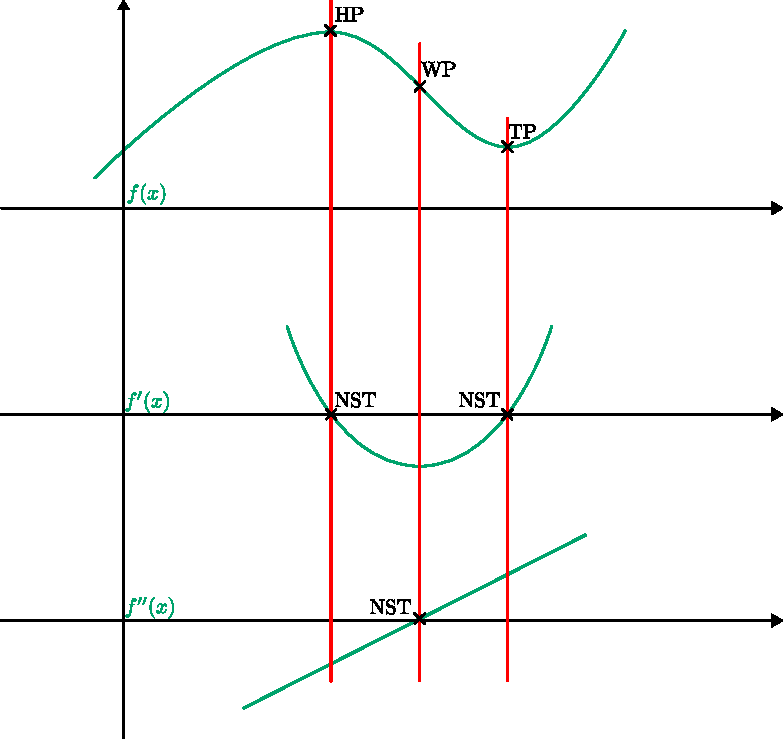
\includegraphics[width=0.8\linewidth]{figures/ableitungsfunktionenskizzieren.pdf} % Pfad anpassen
\end{figure}
\begin{center}
    \crimson{negative} Steigung von $f(x)\iff f'(x)$ verläuft unterhalb der x-Achse
\end{center}
\begin{center}
    \jade{positive} Steigung von $f(x)\iff f'(x)$ verläuft überhalb der x-Achse
\end{center}
\begin{center}
    Extrempunkte von $f(x)\iff$ Nullstellen von $f'(x)\dots$
\end{center}
}

\subsection{Extremwerte und Wendepunkte}

\begin{minipage}{0.5\textwidth}
    \boxx{Extremstellen}{
\begin{equation*}
    f'(x)=0\Rightarrow\text{pot. Extremstellen}
\end{equation*}
\begin{center}
    \begin{tabular}{c|c|c}
        $f''(x)>0$ & Minimum & Lcinksgekrümmt\\
        \hline
        $f''(x)<0$ & Maximum & Rechtsgekrümmt\\
    \end{tabular}
\end{center}
}
\end{minipage}
\begin{minipage}{0.5\textwidth}
    \boxx{Wendestellen}{
\begin{equation*}
    f''(x)=0\Rightarrow\text{pot. Wendestellen}
\end{equation*}
\begin{center}
    \begin{tabular}{c|c}
        $f'''(x)=0$ & pot. Sattelpunkt\\
        \hline
        $f'''(x)\neq0$ & Wendepunkt\\
        \hline
        $f'''(x)>0$ & Rechts-Links Krümmung\\
        \hline
        $f'''(x)<0$ & Links-Rechts-Krümmung\\
    \end{tabular}
\end{center}
}
\end{minipage}


\subsection{Ganzrationale Funktionen}

\boxx{Form}{
\begin{equation*}
    f(x)=a_nx^n+a_{n-1}x^{n-1}+\dots+a_1x+a_0
\end{equation*}
\begin{center}
    Die höchste Potenz einer Ganzrationalen Funktion gibt ihren Grad, und gleichzeitig die miaxmale Anzahl ihrer Nullstellen an
\end{center}
\begin{minipage}{0.33\textwidth}
    \begin{center}
        \begin{tikzpicture}[scale=0.5]
            \begin{axis}[
                xlabel={$x$}, ylabel={$y$},
                ticks=none,
                xmin=-2, xmax=2, ymin=-2, ymax=2,
                samples=100,
                axis y line=center, axis x line=middle, domain=-2:2, legend pos=north east,
                ]
                \addplot [crimson, thick]{x};
                \addlegendentry{$x$};
                \node at (axis cs:1,-1.8) {\crimson{Grad 1}};
            \end{axis}
        \end{tikzpicture}
    \end{center}
\end{minipage}
\begin{minipage}{0.33\textwidth}
    \begin{center}
        \begin{tikzpicture}[scale=0.5]
            \begin{axis}[
                xlabel={$x$}, ylabel={$y$},
                ticks=none,
                xmin=-2, xmax=2, ymin=-2, ymax=2,
                samples=100,
                axis y line=center, axis x line=middle, domain=-2:2, legend pos=north east,
                ]
                \addplot [crimson, thick]{x^2};
                \addlegendentry{$x^2$};
                \node at (axis cs:1,-1.8) {\crimson{Grad 2}};
            \end{axis}
        \end{tikzpicture}
    \end{center}
\end{minipage}
\begin{minipage}{0.33\textwidth}
    \begin{center}
        \begin{tikzpicture}[scale=0.5]
            \begin{axis}[
                xlabel={$x$}, ylabel={$y$},
                ticks=none,
                xmin=-2, xmax=2, ymin=-2, ymax=2,
                samples=100,
                axis y line=center, axis x line=middle, domain=-2:2, legend pos=north east,
                ]
                \addplot [crimson, thick]{x^3};
                \addlegendentry{$x^3$};
                \node at (axis cs:1,-1.8) {\crimson{Grad 3}};
            \end{axis}
        \end{tikzpicture}
    \end{center}
\end{minipage}

\vspace{\baselineskip}

\begin{minipage}{0.33\textwidth}
    \begin{center}
        \begin{tikzpicture}[scale=0.5]
            \begin{axis}[
                xlabel={$x$}, ylabel={$y$},
                ticks=none,
                xmin=-2, xmax=2, ymin=-2, ymax=2,
                samples=100,
                axis y line=center, axis x line=middle, domain=-2:2, legend pos=north east,
                ]
                \addplot [crimson, thick]{x^4};
                \addlegendentry{$x^4$};
                \node at (axis cs:1,-1.8) {\crimson{Grad 4}};
            \end{axis}
        \end{tikzpicture}
    \end{center}
\end{minipage}
\begin{minipage}{0.33\textwidth}
    \begin{center}
        \begin{tikzpicture}[scale=0.5]
            \begin{axis}[
                xlabel={$x$}, ylabel={$y$},
                ticks=none,
                xmin=-2, xmax=2, ymin=-2, ymax=2,
                samples=100,
                axis y line=center, axis x line=middle, domain=-2:2, legend pos=north east,
                ]
                \addplot [crimson, thick]{x^5};
                \addlegendentry{$x^5$};
                \node at (axis cs:1,-1.8) {\crimson{Grad 5}};
            \end{axis}
        \end{tikzpicture}
    \end{center}
\end{minipage}
\begin{minipage}{0.33\textwidth}
    \begin{center}
        \begin{tikzpicture}[scale=0.5]
            \begin{axis}[
                xlabel={$x$}, ylabel={$y$},
                ticks=none,
                xmin=-2, xmax=2, ymin=-2, ymax=2,
                samples=100,
                axis y line=center, axis x line=middle, domain=-2:2, legend pos=north east,
                ]
                \addplot [crimson, thick]{x^6};
                \addlegendentry{$x^6$};
                \node at (axis cs:1,-1.8) {\crimson{Grad 6}};
            \end{axis}
        \end{tikzpicture}
    \end{center}
\end{minipage}
\begin{center}
    $\cdots$
\end{center}
}

\boxx{Globalverhalten}{
    \begin{center}
        \begin{tabular}{c|c}
            \textcolor{crimson}{Grad} $n$ & \textcolor{jade}{Globalverhalten}\\
            \hline
            $n$ gerade & $x\to\infty=+\infty\,\land\,x\to-\infty=+\infty$\\
            $n$ ungerade & $x\to\infty=+\infty\,\land\,x\to-\infty=-\infty$\\
            \hline
            $n$ gerade und Koeffizient negativ & $x\to\infty=-\infty\,\land\,x\to-\infty=-\infty$\\
            $n$ ungerade und Koeffizient negativ & $x\to\infty=-\infty\,\land\,x\to-\infty=+\infty$\\
        \end{tabular}
    \end{center}
}

\subsection{Funktionsscharen}

\boxx{Form}{
\begin{align*}
    f_k(x)&=k\cdot g(x)\\
    &\quad\dots
\end{align*}
}

\boxx{Ableiten}{
\begin{center}
    Der Parameter wird wie eine beliebige Zahl (Konstante) behandelt und dementsprechd abgeleitet
\end{center}
\vspace{-\baselineskip}
\begin{align*}
    f_k(x)&=x^n+k^2\\
    f_k'(x)&=nx^{n-1}
\end{align*}
}

\boxx{Lösen}{
\begin{center}
    Lösungen einer Funktionsschar sind abhängig von dem Parameter, da eine Funktionsschar eine Menge von Funktionen ist. Lösungen mit Parameter geben also alle möglichen Kurven an
\end{center}
\vspace{-\baselineskip}
\begin{align*}
    f_k'(x)&=x^2-k=0\\
    x&=\pm\sqrt{k}
\end{align*}
}

\boxx{Ortskurve}{
\begin{center}
    Die Ortskurve ist die Menge aller Punkte, die durch die Lösungen der Funktionsschar entstehen
\end{center}
\begin{itemize}
    \item Punkt herausfinden EXT$(-2t\vert 16t^3)$
    \item Parameter elliminieren $x=-2t\Rightarrow t=\dfrac{x}{-2}$
    \item In Funktionswert einsetzen $y=16t^3\Rightarrow y=16\cdot\left(\dfrac{x}{-2}\right)^2=-2x^3$
\end{itemize}
}


\subsection{Exponentialfunktion}

\boxx{Form}{
\def\a{\blaue{a}}
\begin{equation*}
    f(x)=c\cdot\a^x \quad\text{mit } \a>0,\,\a\neq1
\end{equation*}
\begin{center}
    \begin{tabular}{c|c}
        $\a>1$ & exponentielle Zunahme\\
        \hline
        $0<\a<1$ & exponentielle Abnahme\\
    \end{tabular}
\end{center}
\begin{center}
    Keine Nullstellen oberhalb der x-Achse
\end{center}
}

\boxx{Globalverhalten}{
\def\a{\blaue{a}}
\begin{center}
    \begin{tabular}{c|c}
        Basis $\a$ & Globalverhalten\\
        \hline
        $\a >1$ & $x\to\infty=+\infty\,\land\,x\to-\infty=0$\\
        $0< \a <1$ & $x\to\infty=0\,\land\,x\to-\infty=+\infty$\\
    \end{tabular}
\end{center}
}

\boxx{Asymptoten}{
\begin{center}
    \begin{tabular}{c|c|c}
        Funktion $f(x)$ & Asymptote & Verhalten\\
        \hline
        $f(x) = \a^x$ & $y=0$ & Die Funktion nähert sich $0$ für $x \to -\infty$\\
         $f(x) = \a^x + \d$ & $y=\d$ & Die Funktion nähert sich $\d$ für $x \to -\infty$\\
         \hline
         $f(x) = \a^x,\,\a < 1$ & $y=0$ & Die Funktion nähert sich $0$ für $x \to \infty$\\
         $f(x) = -\a^x,\,\a < 1$ & $y=0$ & Die Funktion nähert sich $0$ für $x \to \infty$\\
         \hline
         $f(x) = [-]e^{-x}$ & $y=0$ & Die Funktion nähert sich $0$ für $x \to \infty$\\
         $f(x) = e^x + \d$ & $y=\d$ & Die Funktion nähert sich $\d$ für $x \to -\infty$\\
    \end{tabular}
\end{center}
}

\boxx{e-Funktion}{
\begin{center}
    $e\approx2.718\dots$, Euler'sche Zahl
\end{center}

\boxxx{
    \begin{minipage}{0.5\textwidth}
        \vspace{-\baselineskip}
        \begin{gather*}
            f(x)=e^x\\
            f'(x)=e^x\\
            F(x)=e^x
        \end{gather*}
    \end{minipage}
    \begin{minipage}{0.5\textwidth}
        \begin{center}
            \begin{tabular}{c|c}
                $f(x)$ & Ergebnis\\
                \hline
                $e^0$ & 1\\
                $e^1$ & $e$\\
                $e^{\ln(x)}$ & $x$\\
            \end{tabular}
        \end{center}
    \end{minipage}
}


\begin{center}
    $e^x$ wird niemals $=0$. $e^x$ steigt schneller als jede Potenzfunktion. $e^x$ dominiert jede Potenzfunktion
\end{center}

\begin{minipage}{0.5\textwidth}
    \begin{center}
        \dreid{x}{}{-2}{5}{-1}{8, domain=-2:5, ticks=none,legend pos=north east,}{
            \addplot[crimson,thick,samples=100]{e^x};
            \addlegendentry{$e^x$};
            \addplot[jade,thick,domain=-2:5,samples=100]{x^2};
            \addlegendentry{$x^2$};
            \addplot[blaue,thick,samples=100]{2^x};
            \addlegendentry{$2^x$};
            \node at (axis cs:1.5,6) {\crimson{$e^x$}}
            }
    \end{center}
\end{minipage}
\begin{minipage}{0.5\textwidth}
    \boxxx{\begin{center}
        \begin{align*}
            e^{-x}&=\frac{1}{e^x}\\
            e^{-1000}&=\frac{1}{e^{1000}}\\
            \lim_{x\to-\infty}e^x&=0,\,e^x\neq0
        \end{align*}
    \end{center}}
\end{minipage}

\begin{align*}
    f(x)&=e^x(x^2+1)\\
    e^x&\neq0\,\land\,x^2+1=0
\end{align*}
}

\boxx{Logarithmus}{
\begin{center}
    Der Logarithmus ist die Umkehrfunktion der Exponentialfunktion. Wie oft musst du die Basis $\a$ mit sich selbst multiplizieren, um $x$ zu erhalten?
\end{center}
\vspace{-\baselineskip}
\begin{minipage}{0.5\textwidth}
    \begin{align*}
        2^x&=8\\
        \log_2(8)&=x
    \end{align*}
\end{minipage}
\begin{minipage}{0.5\textwidth}
    \begin{equation*}
        a^y=x\quad\text{entspricht}\quad\log_a(x)=y
    \end{equation*}
\end{minipage}
}

\boxx{Natürlicher Logarithmus}{
\begin{center}
    Der natürliche Logarithmus $\ln(x)$ ist die Umkehrfunktion der Exponentialfunktion $e^x$. Der natürliche Logarithmus ist der Logarithmus zur Basis $e$
\end{center}
\vspace{-\baselineskip}
\begin{minipage}{0.5\textwidth}
    \begin{align*}
        \ln(e^x)&=x\\
        e^{\ln(x)}&=x\\
        \ln(1)&=0\\
        \ln(e)&=1\\
    \end{align*}
\end{minipage}
\begin{minipage}{0.5\textwidth}
    \begin{align*}
        \ln(x)&=y\quad\text{genau dann, wenn}\quad e^y=x\\
        f(x)&=\ln(x),\quad f'(x)=\frac{1}{x}
    \end{align*}
\end{minipage}

\boxxline

\begin{center}
    \begin{tabular}{c|c}
        \crimson{Rechenregel} & \\
        \hline
        Produktregel & $\ln(x\cdot y)=\ln(x)+\ln(y)$\\
        Quotientenregel & $\ln\left(\frac{x}{y}\right)=\ln(x)-\ln(y)$\\
        Potenzregel & $\ln(x^y)=y\cdot\ln(x)$\\
    \end{tabular}
\end{center}
}

\boxx{Anwendung von Exponentialfunktionen}{
\begin{itemize}
    \item Exponentielles Wachstum: $f(t)=f(0)\cdot e^{k\cdot t}$
    \item Halbwertszeit: $T_H=\dfrac{1}{k}\cdot\ln\left(\dfrac{1}{2}\right)=-\dfrac{1}{k}\cdot\ln(2)$
    \item Verdopplungszeit: \begin{align*}
        f(T_v)=f(0)\cdot2&=f(0)\cdot e^{kT_v}\\
        e^{kT_v}&=2\quad T_v=\dfrac{1}{k}\cdot\ln(2)
    \end{align*}
\end{itemize}
}

\pagebreak

\subsection{Integrale}

\boxx{Stammfunktion}{
\begin{align*}
    \int f(x)\,dx&=F(x)+C\\
    F(x)&=\a\cdot\dfrac{1}{n+1}\cdot x^{n+1}+C
\end{align*}
\begin{equation*}
    F(x)\leftarrow f(x)\rightarrow f'(x)
\end{equation*}
\begin{center}
    "Aufleiten" wird ungerne gehört. Stattdessen: "Stammfunktion bilden" oder "Integrieren"
\end{center}
}

\boxx{Flächenberechnung}{
\begin{center}
     Die Fläche unter einer Funktion $f(x)$ über einem Intervall $[a,b]$ wird berechnet durch:
\end{center}
\vspace{-\baselineskip}
\begin{align*}
    \int_{a}^{b}f(x)\,dx&=\left[F(x)\right]_{a}^{b}\\
    &=F(b)-F(a)
\end{align*}
\begin{center}
     Die Fläche zwischen zwei Funktionen $f(x)$ und $g(x)$ über einem Intervall $[a,b]$ wird berechnet durch:
\end{center}
\begin{align*}
    \int_{a}^{b}(f(x)-g(x))\,dx&=\left[F(x)-G(x)\right]_{a}^{b}=\left[F(b)-F(a)\right]-\left[G(b)-G(a)\right]\\
    \int_{a}^{b}(f(x)-g(x))\,dx&=\int_{a}^{b}f(x)\,dx-\int_{a}^{b}g(x)\,dx
\end{align*}
}

\boxx{Fallunterscheidung}{
\begin{center}
    Fläche unter einer Funktion $f(x)$:
\end{center}
\begin{center}
    \begin{tabularx}{\textwidth}{>{\centering\arraybackslash}X|>{\centering\arraybackslash}X|>{\centering\arraybackslash}X}
        Situation & Formel & \\
        \hline
        $f(x)\geq0$ auf $[a;b]$ & $A=\int_{a}^{b}f(x)\,dx$ & Keine Betragstriche nötig, da $f(x)\geq0$\\
        \hline
        $f(x)\leq0$ auf $[a;b]$ & $A=\vert\int_{a}^{b}f(x)\,dx\vert$ & Betragstriche nötig, da $f(x)\leq0$\\
        \hline
        $f(x)$ wechselt Vorzeichen & $A=\int_{a}^{b}f(x)\,dx+\vert\int_{b}^{c}f(x)\vert$ & Die Grenzen sind die Nullstellen von $f(x)$\\
    \end{tabularx}
\end{center}

\boxxline

\begin{center}
    Fläche zwischen zwei Funktionen $f(x)$ und $g(x)$:
\end{center}
\begin{center}
    \begin{tabularx}{\textwidth}{>{\centering\arraybackslash}X|>{\centering\arraybackslash}X|>{\centering\arraybackslash}X}
        Situation & Formel & \\
        \hline
        $f(x)\geq g(x)$ auf $[a;b]$ & $ A=\vert\int_{a}^{b}(f(x)-g(x))\,dx\vert$ & $f(x)$ und $g(x)$ schneiden sich nicht\\
        \hline
        $f(x)$ und $g(x)$ schneiden sich & $A=\vert\int_{a}^{b}(f(x)-g(x))\,dx\vert+\vert\int_{b}^{c}(f(x)-g(x))\,dx\vert$ & Die Grenzen sind die Schnittpunkte von $f(x)$ und $g(x)$.\\
    \end{tabularx}
\end{center}

\boxxline

\begin{center}
    Symmetrische Flächen:
\end{center}
\begin{center}
    \begin{tabularx}{\textwidth}{>{\centering\arraybackslash}X|>{\centering\arraybackslash}X|>{\centering\arraybackslash}X}
        Situation & Formel & \\
        \hline
        Achsensymmetrisch & $A=2\cdot\int_{0}^{a}f(x)\,dx$ & $f(x)$ ist Achsensymmetrisch\\
        \hline
        Punktsymmetrisch & $A=2\cdot\int_{0}^{a}\vert f(x)\vert\,dx$ & $f(x)$ ist Punktsymmetrisch\\
    \end{tabularx}
\end{center}
}

\boxx{Rechenregeln}{
\begin{center}
    \begin{tabular}{c|c}
        \crimson{Regel} & \jade{Funktion} $f(x)$\\
        \hline
        Faktorregel & $\int c\cdot f(x)\,dx=c\cdot\int f(x)\,dx$\\
        Summenregel & $\int\left(f(x)+g(x)\right)\,dx=\int f(x)\,dx+\int g(x)\,dx$\\
        Differenzregel & $\int\left(f(x)-g(x)\right)\,dx=\int f(x)\,dx-\int g(x)\,dx$\\
    \end{tabular}
\end{center}
}

\boxx{Uneigentliche Integrale}{
\begin{center}
    Uneigentliche Integrale berechnen unendliche Flächen mit endlichem Flächeninhalt
\end{center}

\boxxline

\begin{center}
    Nach links unendlich:
\end{center}
\begin{equation*}
    \int_{-\infty}^{b}f(x)\,dx=\int_{z}^{b}f(x)\,dx=\lim_{z\to-\infty}\int_{z}^{b}f(x)\,dx
\end{equation*}

\boxxline

\begin{center}
    Nach rechts unendlich:
\end{center}
\begin{equation*}
    \int_{a}^{\infty}f(x)\,dx=\int_{a}^{z}f(x)\,dx=\lim_{z\to\infty}\int_{a}^{z}f(x)\,dx
\end{equation*}

\boxxline

\begin{center}
    In beide Richtungen unendlich:
\end{center}
\begin{equation*}
    \int_{-\infty}^{\infty}f(x)\,dx=\lim_{a\to-\infty}\int_{a}^{0}f(x)\,dx+\lim_{z\to\infty}\int_{0}^{z}f(x)\,dx
\end{equation*}
}

\boxx{Produktintegration}{
\begin{equation*}
    \int f(x) \cdot g(x) \, dx = F(x) \cdot g(x) - \int F(x) \cdot g'(x) \, dx
\end{equation*}
\noindent\rule{\textwidth}{0.4pt}
\begin{center}
    \jade{Vorgehen}
\end{center}
\begin{center}
    Wähle \( f(x) \) und \( g(x) \) so, dass einer der Faktoren einfacher integrierbar (für \( F(x) \)) oder ableitbar (für \( g'(x) \)) ist.
\end{center}
\begin{center}
    Setze \( f(x) \), \( F(x) \), \( g(x) \), und \( g'(x) \) in die Formel ein.
\end{center}
}

\boxx{Rotationskörper}{
\begin{center}
    Ein Rotationskörper entsteht, wenn eine Funktion um die $x$-Achse rotiert wird. Der Rotationskörper hat ein Volumen $V$.
\end{center}
\vspace{-\baselineskip}
\begin{align*}
    V&=\pi\int_{b}^{a}(f(x))^2\,dx\\
    &=\pi\left[F(x)\right]_{a}^{b}=\pi\left[F(b)-F(a)\right]
\end{align*}
\begin{center}
    \dreid{x}{y}{-1}{9}{-3}{3, domain=0:3, xtick={-2,-1,1,2,3,4,5,6,7,8}, ytick={-2,-1,1,2}, legend pos=outer north east,} {
            \addplot[name path=one, jade, thick,domain=0:8]{sqrt(x)};
            \addplot[name path=two, jade, thick,domain=0:8]{-sqrt(x)};
            \addplot[name path=five,domain=0.5:8]{0};
            \addplot[fill=blue!50, opacity=0.5] fill between[of=one and two, soft clip={domain=0:8}];
        }
\end{center}
}

\subsection{Analysis Aufgaben}

\boxx{Steckbriefaufgaben}{
\begin{itemize}
    \item ganzrationale Funktionen bestimmten
    \item Grad \& Eigenschaften festlegen
    \item LGS bilden \& lösen
    \item Werte in $f(x)$ einsetzen
\end{itemize}
}

\boxx{Extremwertproblem mit Nebenbedingung}{
\begin{itemize}
    \item Extremabedingung (Hauptbedingung): $A=a\cdot b$
    \item Nebendingung: Variablen einsetzen: $2a+b=50$
    \item Zielfunktion: \vspace{-\baselineskip}\begin{align*}
        b&=50-2a\\
        A&=a\cdot(50-2a)\\
    \end{align*}
    \vspace{-3\baselineskip}
    \item je nach Aufgabe Maximum/Minimum bestimmen
\end{itemize}
}

\subsection{Lineare Gleichungssysteme}

\boxx{Form}{
    \begin{equation*}
        \begin{matrix} \text{\rom{1}} \\ \text{\rom{2}} \\ \text{\rom{3}} \\ \end{matrix}\Bigg|\begin{matrix}a-b=4\\2a+b=5\\5a-2b=0\\\end{matrix}\Bigg|
    \end{equation*}
}

\boxx{Gauss-Verfahren}{
    \begin{equation*}
        1.\qquad\begin{matrix} \text{\rom{1}} \\ \text{\rom{2}} \\ \text{\rom{3}} \\ \end{matrix}\Bigg|\begin{matrix} 2x &+&3y&+&z&=&1 \\ 4x&-&y&+&3z&=&11 \\ 3x&+&y&-&z&=&0 \\ \end{matrix}\Bigg|=\begin{pmatrix}
            2 & 3 & 1 & \big| & 1 \\
            \jade{4} & -1 & 3 & \big| & 11 \\
            \jade{3} & 1 & -1 & \big| & 0 \\
          \end{pmatrix}          
    \end{equation*}
    
    \boxxline

    \begin{equation*}
        2.\begin{pmatrix}
            2 & 3 & 1 & \big| & 1 \\
            \jade{4} & -1 & 3 & \big| & 11 \\
            \jade{3} & 1 & -1 & \big| & 0 \\
          \end{pmatrix}\xrightarrow{\text{\rom{2}}-2\cdot\text{\rom{1}}}
          \begin{pmatrix}
            2 & 3 & 1 & \big| & 1 \\
            \jade{0} & -7 & 1 & \big| & 9 \\
            3 & 1 & -1 & \big| & 0 \\
          \end{pmatrix}
    \end{equation*}

    \boxxline

    \begin{equation*}
        3.\begin{pmatrix}
            2 & 3 & 1 & \big| & 1 \\
            0 & -7 & 1 & \big| & 9 \\
            3 & 1 & -1 & \big| & 0 \\
          \end{pmatrix}\xrightarrow{\text{\rom{3}}-\frac{3}{2}\cdot\text{\rom{1}}}
          \begin{pmatrix}
            2 & 3 & 1 & \big| & 1 \\
            \jade{0} & -7 & 1 & \big| & 9 \\
            \jade{0} & -\crimson{\frac{7}{2}} & -\frac{5}{2} & \big| & -\frac{3}{2} \\
          \end{pmatrix}
    \end{equation*}

    \boxxline

    \begin{equation*}
        4.\begin{pmatrix}
            2 & 3 & 1 & \big| & 1 \\
            0 & -7 & 1 & \big| & 9 \\
            0 & -\crimson{\frac{7}{2}} & -\frac{5}{2} & \big| & -\frac{3}{2} \\
          \end{pmatrix}\xrightarrow{\text{\rom{3}}-\frac{1}{2}\cdot\text{\rom{2}}}
          \begin{pmatrix}
            2 & 3 & 1 & \big| & 1 \\
            \jade{0} & -7 & 1 & \big| & 9 \\
            \jade{0} & \jade{0} & -3 & \big| & -6 \\
          \end{pmatrix}
    \end{equation*}

    \boxxline

    \begin{equation*}
        5.\qquad\begin{matrix} \text{\rom{1}} \\ \text{\rom{2}} \\ \text{\rom{3}} \\ \end{matrix}\Bigg|\begin{matrix} 2x & + & 3y & + & z & = & 1 \\ & - & 7y & + & z & = & 9 \\ &  &  & - & 3z & = & -6 \\ \end{matrix}\Bigg|
    \end{equation*}
}
 
\section{Algebra}

\subsection{Vektoren}

\boxx{Form}{
    \begin{equation*}
        \vec{AB}\begin{pmatrix}
            b_1-a1\\
            b_2-a_2\\
            b_3-a_3
        \end{pmatrix}
    \end{equation*}
}

\boxx{Vektoren Addieren \& Subtrahieren}{
    \begin{center}
        Addition:
    \end{center}
    \begin{equation*}
        \vec{a}+\vec{b}=\begin{pmatrix}
            a_1+b_1\\
            a_2+b_2\\
            a_3+b_3
        \end{pmatrix}
    \end{equation*}
    \begin{center}
        Subtraktion:
    \end{center}
    \begin{equation*}
        \vec{a}-\vec{b}=\begin{pmatrix}
            a_1-b_1\\
            a_2-b_2\\
            a_3-b_3
        \end{pmatrix}
    \end{equation*}
}

\boxx{Betrag eines Vektors}{
    \begin{equation*}
        |\vec{a}|=\sqrt{a_1^2+a_2^2+a_3^2}
    \end{equation*}
}

\vspace{\baselineskip}

\hspace{-0.6cm}\minipagee{0.5}{\boxx{Skalarprodukt}{
    \begin{equation*}
        \vec{a}\circ\vec{b}=a_1b_1+a_2b_2+a_3b_3
    \end{equation*}
    \begin{equation*}
        \vec{a}\perp\vec{b}\iff\vec{a}\cdot\vec{b}=0
    \end{equation*}
}
}
\minipagee{0.5}{\boxx{Kollinearität}{
    \begin{equation*}
        \vec{a}\cdot k=\begin{pmatrix}
            a_1\cdot k\\
            a_2\cdot k\\
            a_3\cdot k
        \end{pmatrix}
    \end{equation*}
    Ist ein Vektor das Vielfache vom anderen, so haben beide die gleiche Richtung, aber unterschiedliche Längen
}}

\vspace{\baselineskip}

\boxx{Kreuzprodukt}{
    \minipagee{0.5}{\begin{equation*}
        \vec{a}\times\vec{b}=\begin{pmatrix}
            a_2\cdot b_3-b_2\cdot a_3\\
            a_3\cdot b_1-b_3\cdot a_1\\
            a_1\cdot b_2-b_1\cdot a_2
        \end{pmatrix}=\vec{n}
    \end{equation*}}
    \minipagee{0.5}{
        \begin{figure}[H] % Verhindert Gleitverhalten
            \centering
            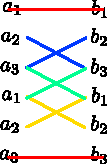
\includegraphics[width=0.2\linewidth]{figures/Kreuzprodukt.pdf} % Pfad anpassen
        \end{figure}
    }

    \begin{equation*}
        \vec{n}\perp\vec{a},\vec{b}\qquad\vec{n}=\text{Normalenvektor}
    \end{equation*}
}

\boxx{Lagebeziehungen}{
    \begin{equation*}
        x=y = \begin{matrix}\text{\rom{1}}\\\text{\rom{2}}\\\text{\rom{3}}\end{matrix}\Bigg|\begin{matrix}x_1=y_1\\x_2=y_2\\x_3=y_3\end{matrix}\Bigg|
    \end{equation*}
    \begin{tabularx}{\textwidth}{>{\centering\arraybackslash}X|>{\centering\arraybackslash}X|>{\centering\arraybackslash}X|>{\centering\arraybackslash}X}
        Lagebeziehung & keine Lösung & eine Lösung & unendlich viele Lösungen\\
        \hline
        Gerade:Gerade & echt Parallel & Schnittpunkt & identisch ($g_1=g_2$)\\
        Gerade:Ebene & echt Parallel & Schnittpunkt & identisch ($g\in E$)\\
        Ebene:Ebene & echt Parallel & Schnittgerade & identisch ($E_1=E_2$)\
    \end{tabularx}
}

\boxx{Schnittwinkel}{
    \begin{tabularx}{\textwidth}{>{\centering\arraybackslash}X|>{\centering\arraybackslash}X|>{\centering\arraybackslash}X}
        Schnittwinkel & trig. & $\alpha$\\
        \hline
        Gerade : Gerade & $\cos(\alpha)=\dfrac{\left|\vec{a}\circ\vec{b}\right|}{\left|\vec{a}\right|\cdot|\vec{b}|}$ & $\alpha=\cos^{-1}\left(\dfrac{\left|\vec{a}\circ\vec{b}\right|}{\left|\vec{a}\right|\cdot|\vec{b}|}\right)$\\
        \hline
        \hline
        Gerade : Ebene & $\cos(\alpha)=\dfrac{\left|\vec{a}\circ\vec{n}\right|}{\left|\vec{a}\right|\cdot|\vec{n}|}$ & $\alpha=\cos^{-1}\left(\dfrac{\left|\vec{a}\circ\vec{n}\right|}{\left|\vec{a}\right|\cdot|\vec{n}|}\right)$\\
        \hline
        \hline
        Ebene : Ebene & $\sin(\alpha)=\dfrac{\left|\vec{n_1}\circ\vec{n_2}\right|}{\left|\vec{n_1}\right|\cdot|\vec{n_2}|}$ & $\alpha=\sin^{-1}\left(\dfrac{\left|\vec{n_1}\circ\vec{n_2}\right|}{\left|\vec{n_1}\right|\cdot|\vec{n_2}|}\right)$
    \end{tabularx}
    \begin{center}
        $\left|\qquad\right|=\text{kleinerer Winkel}$ und $\vec{a},\vec{b}=\text{Richtungsvektoren}$ und $\vec{n}=\text{Normalenvektor}$
    \end{center}
}

\subsection{Geraden}

\boxx{Geradengleichung}{
    \begin{equation*}
        g:\vec{x} = 
        \underbrace{\begin{pmatrix}
        a_1\\
        a_2\\
        a_3
        \end{pmatrix}}_{\text{Stützvektor}}
        +t\cdot 
        \underbrace{\begin{pmatrix}
        b_1\\
        b_2\\
        b_3
        \end{pmatrix}}_{\text{Richtungsvektor}}
    \qquad\qquad t \in \mathbb{R}
    \end{equation*}
}

\boxx{Lagebeziehung}{
    \begin{figure}[H] % Verhindert Gleitverhalten
        \centering
        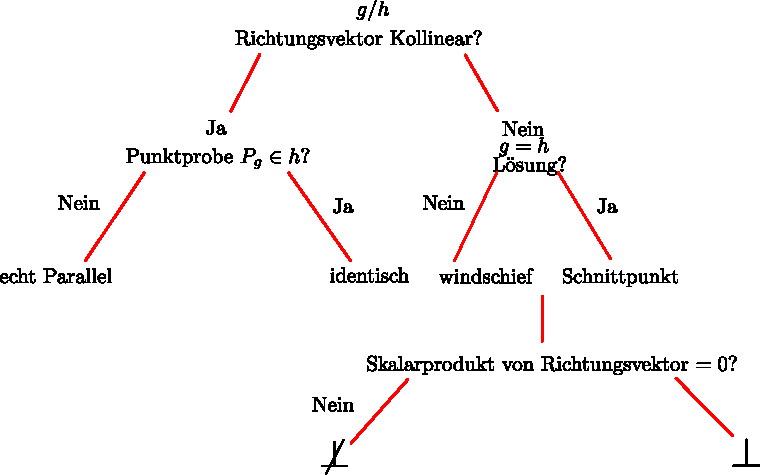
\includegraphics[width=0.8\linewidth]{figures/Lagebeziehung.pdf} % Pfad anpassen
    \end{figure}
}

\boxx{Abstand Gerade:Gerade}{
    \begin{align*}
        g:\vec{x}&=\vec{p}+t\cdot\vec{u} &h:\vec{x}=\vec{q}+s\cdot\vec{v}\\
        \vec{u}&\times\vec{v}=\vec{n} &E\in g
    \end{align*}
    \begin{center}
        $E$ mit $\vec{n}$ aufstellen\\
        $p$ in $E$ einsetzen und d (Koordinatenform) bestimmen
    \end{center}
    \begin{equation*}
        \text{neue Gerade: }\vec{x}=\vec{q}+r\cdot\vec{n}
    \end{equation*}
    \begin{center}
        $\left|\vec{FQ}\right|$ bestimmen
    \end{center}
}


\boxx{Abstand (Lotfußpunkt) Gerade:Punkt}{
    \minipagee{0.5}{
        \begin{center}
            $E=$ Hilfsebene, $g=$ Gerade, $A=$ Punkt
        \end{center}
        \begin{equation*}
            E:\vec{x}=n_1x_1+n_2x_2+n_3x_3=d,\quad\vec{n}=RV\text{ von }g
        \end{equation*}
        \begin{center}
            $A$ in $E$ einsetzen und d berechnen
        \end{center}
        \begin{center}
            $g$ in $E$ einsetzen und $t$ berechnen
        \end{center}
    }
    \minipagee{0.5}{
        \begin{center}
            Orthogonalität: $g:\vec{x}=\underbrace{\begin{pmatrix}c_1\\c_2\\c_3\end{pmatrix}}_{\text{Punkt A}}+t\cdot\begin{pmatrix}b_1\\b_2\\b_3\end{pmatrix}\qquad t\in\mathbb{R}$
        \end{center}
        \begin{equation*}
            \vec{F}=\begin{pmatrix}
                c_1+b_1\cdot t\\
                c_2+b_2\cdot t\\
                c_3+b_3\cdot t
            \end{pmatrix}
        \end{equation*}
        \begin{equation*}
            \vec{AF}\circ\vec{RV}=0
        \end{equation*}
        \begin{equation*}
            \left(c_1+b_1\cdot t\right)\cdot{RV}_1+\left(c_2+b_2\cdot t\right)\cdot{RV}_2+\left(c_3+b_3\cdot t\right)\cdot{RV}_3
        \end{equation*}
        \begin{center}
            $t$ berechnen\\
            $t$ in $g$ einsetzen und $F$ bestimmen
        \end{center}
        \begin{equation*}
            \left|\vec{AF}\right|=\text{kleinster Abstand}
        \end{equation*}
    }
}

\subsection{Ebenen}

\minipagee{0.5}{\boxx{Parameterform}{
    \begin{equation*}
        E:\vec{x}=\underbrace{\begin{pmatrix}
            a_1\\
            a_2\\
            a_3
        \end{pmatrix}}_{\text{Stützvektor}}+r\cdot\underbrace{\begin{pmatrix}
            b_1\\
            b_2\\
            b_3
        \end{pmatrix}}_{\text{Spannvektor}}+s\cdot\underbrace{\begin{pmatrix}
            c_1\\
            c_2\\
            c_3
        \end{pmatrix}}_{\text{Spannvektor}}
    \end{equation*}
}}
\minipagee{0.5}{\boxx{Begrenzung von Ebenen}{
    \begin{center}
        \begin{tikzpicture}[scale=0.5]
            \begin{axis}[
                xlabel={$SV_2$}, ylabel={$SV_1$},
                ticks=none,
                xmin=0, xmax=5, ymin=0, ymax=5, axis lines=middle,
                ]
                \draw[crimson,dashed] (0,5) -- (5,0);
                \draw[jade,thick,dashed] (0,5) -- (5,5) -- (5,0);
            \end{axis}
        \end{tikzpicture}
    \end{center}
    \vspace{-\baselineskip}
    \begin{align*}
        &\crimson{r+s\leq 1}\quad r,s\in\mathbb{R}^+\\
        &\jade{0\leq r,s\leq 1}
    \end{align*}
}}

\boxx{Koordinatenform}{
    \begin{equation*}
        E:ax_1+bx_2+cx_3=d,\quad\begin{pmatrix}
            a\\
            b\\
            c
        \end{pmatrix}=\vec{n}\quad(\text{Kreuzprodukt beider Spannvektoren})
    \end{equation*}
    \begin{center}
        Für $d$ einen Punkt in die Ebene einsetzen
    \end{center}
}

\boxx{Hesse'sche Normalform}{
    \begin{equation*}
        E:\left(\vec{x}-\vec{p}\right)\cdot\vec{n_0}=0
    \end{equation*}
    \begin{center}
        Wobei $\left(\vec{x}-\vec{p}\right)$ ein Verbindungsvektor zwischen zwei Punkten auf der Ebene, und $\vec{n_0}$ der normierte Normalenvektor ist
    \end{center}
    \begin{center}
        Einen Vektoren normiert man, indem man ihn durch seine Länge teilt. Dadurch wird nur noch seine Richtung angegeben:
    \end{center}
    \begin{equation*}
        \vec{n_0}=\dfrac{1}{|\vec{n}|}\cdot\vec{n}
    \end{equation*}

    \boxxline

    \begin{center}
        \jade{Abstand Punkt:Ebene}
    \end{center}
    \begin{equation*}
        \text{Abstand}=\dfrac{ax_1+bx_2+cx_3-d}{\vec{n}}
    \end{equation*}
}



\boxx{Abstand Ebene:Punkt}{
    \begin{center}
        $\vec{n}$ von $E$ bilden
    \end{center}
    \begin{center}
        neue Gerade $g$ mit $\vec{n}$ und Punkt $P$ als Stützvektor
    \end{center}
    \begin{center}
        $E=g\to$ Schnittpunkt $F$
    \end{center}
    \begin{center}
        $\left|\vec{FP}\right|=\text{Abstand}$
    \end{center}
}

\boxx{Abstand Ebene:Gerade}{
    \begin{center}
        $P\in g\to$ Abstand Ebene:Punkt
    \end{center}
}

\boxx{Abstand Ebene:Ebene}{
    \begin{center}
        $P\in E\to$ Abstand Ebene:Punkt
    \end{center}
}

\section{Stochastik}

\subsection{Baumdiagramm}

\boxx{Diagramm}{
    \begin{center}
        Aufgabe: Unter den Abonnenten sind $70\%$ höchstens $40$ Jahre als. Von diesen haben $80\%$ das Komplettpaket gewählt. Unter denjenigen Abonnenten, die älter sind als $40$ Jahre, haben sich $50\%$ für das Komplettpaket entschieden
    \end{center}

    \boxxline

    \begin{figure}[H] % Verhindert Gleitverhalten
        \centering
        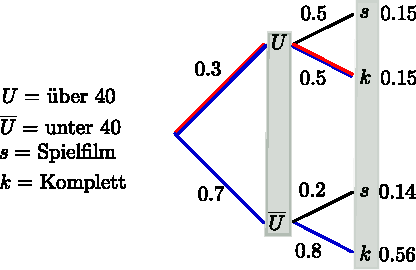
\includegraphics[width=0.8\linewidth]{figures/Baumdiagramm.pdf} % Pfad anpassen
    \end{figure}
}

\boxx{Pfadregel}{
        \begin{equation*}
            \text{\textcolor{graue}{Pfadregeln: }}\hspace{-0.2cm}\underbrace{P(U\cap s)}_{U40+\text{Spielfilm}}=0.3\cdot0.5=\hspace{-0.5cm}\underbrace{P_U(k)=\frac{2}{3}}_{\text{Komplettpaket für }U40}
        \end{equation*}
}

\boxx{Produktregel}{
    \begin{center}
        \crimson{Produktregel:} Wahrscheinlichkeit \crimson{einen bestimmten Versuchsausgang} zu erhalten, also die Wahrscheinlichkeit, dass eine Person über $40$ ist, und das Komplettpaket hat $0.3\cdot0.5=0.15$
    \end{center}
}

\boxx{Summenregel}{
    \begin{center}
        \blaue{Summenregel:} Wahrscheinlichkeit \blaue{mehrere Versuchsausgänge} zu erhalten, also die Wahrscheinlichkeit, dass das Komplettpaket gebucht wurde $0.3\cdot0.5+0.7\cdot0.8=0.71$
    \end{center}
}

\pagebreak

\subsection{Vierfeldertafel}

\boxx{Diagramm}{
    \begin{figure}[H] % Verhindert Gleitverhalten
        \centering
        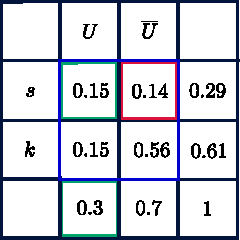
\includegraphics[width=0.5\linewidth]{figures/Vierfeldertafel.pdf} % Pfad anpassen
    \end{figure}
    \begin{center}
        Hilfe zur Berechnung von Ereignissen
    \end{center}
    \begin{equation*}
        \text{\textcolor{blaue}{geschnittene Wahrscheinlichkeit}}
    \end{equation*}
    \begin{equation*}
        \crimson{P(\overline{U}\cap s)}=0.14
    \end{equation*}
    \begin{center}
        \jade{bedingte Wahrscheinlichkeit}
        \begin{equation*}
            P_U(s)=\dfrac{P(U\cap s)}{P(U)}\qquad\frac{0.15}{0.3}=50\%
        \end{equation*}
        Leute die das Spiefilmpaket gekauft haben unter denen, die $40$ Jahre alt sind
    \end{center}
}

\subsection{Wahrscheinlichkeitsverteilung}

\boxx{Variablen}{
    \begin{center}
        \begin{tabularx}{\textwidth}{>{\centering\arraybackslash}X|>{\centering\arraybackslash}X}
            $n$ & Anzahl der ausgeführten Versuche oder Durchführungen \\
            \hline
            $p$ & Trefferwahrscheinlichkeit im Versuch \\
            \hline
            $X$ & Zufallsvariable \\
            \hline
            $\mu$ & Erwartungswert von $X$, $\mu=x_1\cdot P(X=x_1)+x_2\cdot P(X=x_2)+\dots$ \\
            \hline
            $\sigma$ & Standardabweichung von $X$, $\sigma=\sqrt{\left(x^1-\mu\right)^2\cdot P\left(X=x_1\right)+\dots}$ \\
        \end{tabularx}            
    \end{center}
}

\subsection{Bernoulli Versuch}

\boxx{Bernoulli-Formel}{
    \begin{equation*}
        P(X=k)=\binom{n}{k}\cdot p^k\cdot (1-p)^{n-k}\qquad\text{die Wahrscheinlichkeit für genau $k$ Erfolge in $n$ Versuchen}
    \end{equation*}
}

\boxx{Bernoullikoeffizient}{
    \begin{equation*}
        \binom{n}{k}\qquad\text{Anzahl, dass in $n$ Versuchen $k$ Erfolge eintreten}
    \end{equation*}
}

\boxx{Beispiel}{
    \begin{center}
        Es gibt drei Blutgruppen: O, A, B, AB. $41\%$ haben O. Es kommen $80$ Spender. 
    \end{center}
    \minipagee{0.5}{
        \begin{equation*}
            X=\text{Anzahl der Blutspender mit O}
        \end{equation*}
    }
    \minipagee{0.5}{
        \begin{align*}
            n&=80\\
            p&=0.41
        \end{align*}
    }
    
    \boxxline
    \vspace{\baselineskip}

    \minipagee{0.4}{
        \begin{itemize}
            \item Genau $25$ Spender haben O \begin{align*}
                P(X=25)&=1.9\%\\
                \text{binomPdf}(80;0.41;25)&=0.018917
            \end{align*}
            \item höchstens $20$ Spender haben O \begin{align*}
                P(X\leq20)&=0.2\%\\
                \text{binomCdf}(80;0.41;0;20)&=0.002061
            \end{align*}
            \item mindestens $30$ Spender haben O \begin{align*}
                P(X\geq30)&=72.2\%\\
                \text{binomCdf}(80;0.41;30;80)&=0.772405
            \end{align*}
        \end{itemize}
    }
}

\subsection{Kenngrößen}

\boxx{n}{
    \begin{center}
        Eine Maschine arbeitet nicht präzise. $3\%$ der Produkte sind mangelhaft. Wie viele Produkte müssen geprüft werden, dass mit $99\%$ Wahrscheinlichkeit ein Produkt mangelhaft ist?
    \end{center}
    \minipagee{0.5}{
        \begin{align*}
            X&=\text{Anzahl der mangelhaften Produkte}\\
            n&=?\\
            p&=0.03\qquad P(X\geq1)\geq99
        \end{align*}
    }
    \minipagee{0.5}{
        \begin{equation*}
            \dfrac{\ln(0.01)}{\ln(0.03)}=151.191\,\text{Produkte müssen geprüft werden}
        \end{equation*}
    }
}

\boxx{p}{    
    \begin{center}
        Ein Weihnachtskalender mit $24$ Türchen hat verschiedene Schokoladensorten. Was ist die Mindesterfolgswahrscheinlichkeit, mit der eine Sorte drin sein muss, sodass diese mit mindestens $95\%$ Wahrscheinlichkeit mindestens ein mal im Kalender ist?
    \end{center}
    \minipagee{0.5}{
        \begin{align*}
            X&=\text{Anzahl der Tafeln einer Sorte}\\
            n&=24
        \end{align*}
    }
    \minipagee{0.5}{
        \begin{equation*}
            1-\sqrt[24]{0.05}=0.117346\,\text{mit }11.8\%\text{ ist sie enthalten}
        \end{equation*}
    }
}

\boxx{k}{
    \begin{center}
        Für eine Studie wurden $500$ Personen genötigt. Nur $75\%$ der befragten wollen daran teilnehmen. Wie viele Personen müssen befragt werden, dass zu $95\%$ $500$ Leute zur Auskunft bereit werden?
    \end{center}
    \minipagee{0.5}{
        \begin{align*}
            X&=\text{Anzahl der befragten Personen}\\
            p&=0.75\\
            k&\geq500
        \end{align*}
    }
    \minipagee{0.5}{
        \begin{align*}
            \text{binomCdf}&(700;0.75;0;499)\\
            \text{binomCdf}&(690;0.75;0;499)\\
            \text{binomCdf}&(692;0.75;0;499)\\
            \text{binomCdf}&(692;0.75;500;592)=0.955
        \end{align*}
    }
}

\subsection{Mu und Sigma}

\boxx{Erwartungswert einer binomialverteilten Zufallsgröße}{
    \begin{equation*}
        \mu=n\cdot p
    \end{equation*}
}

\subsection{Standardabweichung}

\boxx{Standardabweichung einer binomialverteilten Zufallsgröße}{
    \begin{equation*}
        \sigma=\sqrt{n\cdot p\cdot (1-p)}
    \end{equation*}
}

\subsection{Normalverteilung}

\boxx{Beispiel}{
    \begin{center}
        Körpergrößen können näherungsweise mithilfe einer normalverteilten Zufallsgröße modelliert werden. Es ergibt sich für die Körpergröße von $18$ bis $20$-jährigen Frauen ein Mittelwert von $1.68$m bei einer Standardabweichung von $6.5$cm
    \end{center}
    \begin{center}
        $X=$Körpergröße $18$ bis $20$-jähriger Frauen\\
        $\mu=1.68$cm$\qquad\sigma=6.5$cm
    \end{center}
    \vspace{-\baselineskip}
    \begin{align*}
        \text{kleiner als }1.65=P(X<165)=\text{normCdf}(-\infty;165;168;6.5)=0.322206=32.22\%\\
        \text{größer als }1.80=P(X>180)=\text{normCdf}(180;+\infty;168;6.5)=0.032435=3.24\%\\
        \text{zwischen }1.70\text{ und }1.75=P(170\leq X\leq175)=\text{normCdf}(170;175;168;6.5)=0.238401=23.84\%\\
        \text{genau }1.70=P(X=170)=\text{normPdf}(170;168;6.5)=0.058538=5.85\%
    \end{align*}
}

\subsection{Sigmaregeln}

\boxx{$1\sigma,\,2\sigma,\,3\sigma$-Regel}{
    \begin{center}
        Für $\mu=n\cdot p$ und $\sigma=\sqrt{n\cdot p\cdot(1-p)}$ erhält man die Näherung
    \end{center}
    \vspace{-\baselineskip}
    \begin{align*}
        1.&P(\mu-\sigma\leq X\leq\mu+\sigma)=68.3\%\\
        2.&P(\mu-2\sigma\leq X\leq\mu+2\sigma)=95.4\%\\
        3.&P(\mu-3\sigma\leq X\leq\mu+3\sigma)=99.7\%
    \end{align*}
}

\boxx{"glatte" Wahrscheinlichkeiten}{
    \vspace{-\baselineskip}\begin{align*}
        4.&P(\mu-1.64\sigma\leq X\leq\mu+1.64\sigma)=90\%\\
        5.&P(\mu-1.96\sigma\leq X\leq\mu+1.96\sigma)=95\%\\
        6.&P(\mu-2.58\sigma\leq X\leq\mu+2.58\sigma)=99\%
    \end{align*}
}

\subsection{Hypothesentests}

\boxx{linksseitiger Hypothesentest}{
    \begin{center}
        Beispiel:\\
        Max hat einen Würfel $600$-mal geworfen und $87$ mal eine drei erhalten. Du hälst den Würfel für gezinkt. Führe einen linksseitigen Hypothesentest mit einem Signifikanzniveau $\alpha=5\%$ durch. Bestimme sein Ablehnungsbereich und gib eine Entschiedungsregel für dein Ergebnis an.
    \end{center}
    \vspace{-\baselineskip}
    \begin{align*}
        X&=\text{Anzahl der Dreien}\\
        n&=600\\
        p&=\dfrac{1}{6}\\
    \end{align*}
}

\boxx{Nullhypothese}{
    \begin{center}
        $H_0$: Der Würfel ist fair, $p=\dfrac{1}{6}$. Grenze des Ablehnungsbereichs $P(X\leq g)\leq0.05$
    \end{center}
}

\boxx{Alternative}{
    \begin{center}
        $H_1$: Der Würfel ist gezinkt, $p<\dfrac{1}{6}$. Grenze des Ablehnungsbereichs $P(X\leq g)\leq0.05$
    \end{center}
    \begin{center}
        \begin{tabular}{c|c}
            $g$&$P(X\leq g)$\\
            \hline
            $90$&$0.1487$\\
            $85$&$0.0538$\\
            $84$&$0.0424$ (Alpha Fehler)
        \end{tabular}
    \end{center}
    \begin{center}
        Ablehnungsbereich A$[0;84]\to$ hätte er weniger als $84$ gewürfelt wäre die Nullhypothese abgelehnt.
    \end{center}
}

\boxx{Alpha Fehler}{
    \begin{center}
        Wahrscheinlichkeit, dass die Aussage verworfen wird, obwohl man recht hat.
    \end{center}
}

\boxx{Beta Fehler}{
    \begin{center}
        Nullhypothese wird angenommen, obwohl sie abgelehnt hätte werden müssen
    \end{center}
    \vspace{-\baselineskip}
    \begin{align*}
        n&=600\\
        p&=\dfrac{1}{6}\\
    \end{align*}
    \begin{center}
        $0.045$ mit einer Wahrscheinlichkeit von $4\%$ ist der Würfel gezinkt, aber es wurde die falsche Probe genommen bei $84$.
    \end{center}
}

\end{document}